\documentclass[a4paper,12pt]{report}
\usepackage[utf8]{inputenc}
\usepackage[english]{babel}
\usepackage[T1]{fontenc}
\usepackage{graphicx}
\usepackage{geometry}
\usepackage{hyperref}
\usepackage{amsmath}
\usepackage{amssymb}
\usepackage{listings}
\usepackage{xcolor}
\usepackage{caption}
\usepackage{subcaption}
\usepackage{booktabs}
\usepackage{tikz}
\usetikzlibrary{shapes.geometric, arrows, positioning, fit, backgrounds, shadows}
\usepackage[percent]{overpic}

\geometry{
    a4paper,
    total={170mm,257mm},
    left=20mm,
    top=20mm,
}

% Code listing configuration
\lstset{
    basicstyle=\ttfamily\small,
    breaklines=true,
    frame=single,
    numbers=left,
    numberstyle=\tiny,
    captionpos=b
}

% Remove "Chapter" word and keep number on same line as title
\usepackage{titlesec}
\titleformat{\chapter}[hang]
  {\normalfont\huge\bfseries}{\thechapter}{1em}{}

\title{\textbf{Reinforcement Learning for Sim2Real and path following in Isaaclab with Ur10}}
\author{
    \textbf{Auteurs :} \\
    RAFANIAINA Jeovani \\
    Vogelgesang Luca \\[1cm]
    \textbf{Encadrant :} \\
    Nom de l'encadrant
}
\date{\today}

\begin{document}

\begin{titlepage}
    \centering
    \begin{minipage}{0.3\textwidth}
        \centering
        \includegraphics[width=0.9\linewidth]{images/lirmlogo.png}
    \end{minipage}
    \hfill
    \begin{minipage}{0.3\textwidth}
        \centering
        \includegraphics[width=0.9\linewidth]{images/unilogo.jpeg}
    \end{minipage}
    \hfill
    \begin{minipage}{0.3\textwidth}
        \centering
        \includegraphics[width=0.9\linewidth]{images/logoEEA.png}
    \end{minipage}\\[1.5cm]

    {\Huge \textbf{Reinforcement Learning for Sim2Real and Path Following in Isaaclab with UR10} \par}
    
    \vspace{1.5cm}

    {\Large
    \textbf{Authors :} \\
    RAFARANIAINA Jeovani \\
    VOGELGESANG Luca \\[1cm]
    \textbf{Supervisor :} \\
    Chao LIU 
    \par}

    \vspace{1.5cm}

    \textbf{\Large Abstract}\\[0.5cm] 
    \parbox{0.9\linewidth}{
        \begin{abstract}
        This thesis presents the development of a hybrid robotic control pipeline for a UR10 manipulator, combining classical motion planning (MoveIt on ROS 2) with residual reinforcement learning (PPO on Isaac Lab). The system implements a residual learning architecture where a learned policy injects real-time corrections into the nominal trajectory to compensate for calibration errors and perception noise.

        Due to time constraints limiting physical testing, the validation strategy focuses on a rigorous \textbf{Sim-to-Sim} approach using extensive domain randomization to simulate a realistic ``Digital Twin'' of the physical setup. Comparative experiments demonstrate that the proposed residual agent significantly outperforms the standard Open-Loop baseline. Under perturbed conditions, the closed-loop policy reduces the mean tracking error by \textbf{69.7\%} (from 28.4\,mm to 8.6\,mm) and improves consistency by reducing the error standard deviation by \textbf{71.4\%}, providing strong evidence of the system's robustness and its potential for future transfer to the real robot.
        \end{abstract}
    }

    \vfill
    {\large \today \par}
\end{titlepage}

\tableofcontents

\chapter*{Introduction}
\addcontentsline{toc}{chapter}{Introduction}
\section{Contexte}
L'essor de l'apprentissage par renforcement (RL) en robotique et la problématique du "Reality Gap" (l'écart entre simulation et réalité).

\section{Problématique}
Comment garantir un mouvement fluide et précis pour un UR10 en utilisant des données visuelles imparfaites ?

\section{Objectif}
Développer une approche de Residual Reinforcement Learning pour une tâche de reaching planaire (2D).

\section{Annonce du plan}
De la configuration logicielle à la validation Sim-to-Sim.
% - Chapter 2: System architecture (ROS2, Isaac Lab, PPO)
% - Chapter 3: Validation strategy (domain randomization tests)
% - Chapter 4: Experimental results
% - Chapter 5: Conclusion



\chapter{Background \& Key Concepts}
% Chapter 1: Background (~2.5 pages)

\section{Motion Planning and ROS2/MoveIt}

Robotic manipulators like the Universal Robots UR10 are characterized by their kinematic structure. The UR10 is a 6 degrees-of-freedom (DoF) serial manipulator, where each revolute joint contributes one rotational degree of freedom. The relationship between joint angles and end-effector position is described by forward kinematics, while the inverse problem—computing joint configurations to reach a desired pose—is solved through inverse kinematics algorithms.

Motion planning addresses the challenge of computing collision-free trajectories from an initial to a goal configuration. MoveIt, integrated with the Robot Operating System 2 (ROS2), is the de facto standard for motion planning in robotics research and industry. It provides sampling-based planners (e.g., RRT, RRT*) and optimization-based methods (e.g., CHOMP, STOMP) to generate trajectories that respect joint limits, avoid obstacles, and minimize path length or execution time.

However, classical motion planners operate under the assumption that the robot model and environment representation are accurate. When calibration errors exist—such as inaccurate camera extrinsics or AprilTag position uncertainties—MoveIt generates trajectories to the \textit{perceived} target location rather than the true one. The planner has no mechanism to detect or compensate for these systematic errors during execution. This limitation motivates the need for adaptive control strategies that can correct for perception-induced positioning errors in real-time.

\section{Reinforcement Learning for Robotics}

Reinforcement Learning (RL) is a machine learning paradigm where an agent learns to make decisions by interacting with an environment. The agent observes the current state, selects an action according to its policy, receives a reward signal indicating the quality of that action, and transitions to a new state. The learning objective is to maximize the cumulative expected reward over time.

Unlike supervised learning, which requires labeled input-output pairs, RL learns from trial and error through exploration of the state-action space. This makes RL particularly suitable for robotics, where optimal control policies are difficult to manually specify but can be discovered through interaction. However, this advantage comes with a critical challenge: sample efficiency.

Training RL policies on physical robots is prohibitively slow and potentially dangerous. Each policy update requires hundreds or thousands of trajectory rollouts, which would take weeks on a real robot and risk mechanical damage during exploration. GPU-accelerated simulation environments like NVIDIA Isaac Lab address this bottleneck by enabling massive parallelization: instead of running one robot at a time, thousands of simulated environments execute simultaneously on GPU cores, reducing training time from weeks to hours.

The Proximal Policy Optimization (PPO) algorithm has emerged as a popular choice for continuous control in robotics due to its stability and sample efficiency. PPO belongs to the family of policy gradient methods, which directly optimize the policy parameters to maximize expected returns. Its key innovation is a clipped objective function that prevents excessively large policy updates, ensuring stable learning even in high-dimensional continuous action spaces. These properties have made PPO successful in tasks ranging from legged locomotion to dexterous manipulation.

\section{Residual Learning}

Pure end-to-end learning, where an RL policy directly controls all robot joints, faces two significant challenges: safety and training efficiency. Without constraints, the policy might produce unsafe actions during exploration, and learning from scratch requires extensive environment interaction even for tasks where prior knowledge exists.

Residual learning offers an elegant solution by decomposing the control policy into two components: a nominal controller and a learned residual. Mathematically, the final action is expressed as:
\begin{equation}
a_{\text{final}} = a_{\text{nominal}} + a_{\text{residual}}
\end{equation}

In our case, $a_{\text{nominal}}$ is the trajectory generated by MoveIt, which ensures kinematic feasibility and collision avoidance. The learned policy $a_{\text{residual}}$ produces small corrective actions that compensate for errors the nominal controller cannot address—specifically, perception noise and calibration inaccuracies.

This approach provides several advantages. First, \textit{safety}: the nominal controller guarantees that the robot remains within its operational envelope, while the residual is bounded to prevent large deviations. Second, \textit{accelerated learning}: by focusing only on corrections rather than full control, the policy search space is drastically reduced, enabling faster convergence. Third, \textit{interpretability}: when the system fails, it is easier to diagnose whether the issue stems from the planner or the learned component.

Residual reinforcement learning has been successfully applied to various robotic tasks. Johannink et al. (2019) demonstrated residual RL for precise insertion tasks, where a PD controller provided nominal tracking and RL learned contact-rich corrections. Silver et al. (2018) used residual policies to improve helicopter aerobatics beyond classical controllers. Our work extends this paradigm to vision-based manipulation with AprilTag localization, where perception uncertainties are the primary source of error requiring learned compensation.


\chapter{System Architecture}
\section{System Architecture}

This chapter provides an overview of the complete system architecture before diving into implementation details. We first present the global software pipeline connecting all components, then describe the physical hardware setup, and finally explain the coordinate transformation framework that enables precise motion planning.

\subsection{Global Software Pipeline}

Figure \ref{fig:global_pipeline} presents the complete data flow from the physical setup to validation. This pipeline consists of five key stages, each playing a specific role in the residual reinforcement learning approach.

\begin{figure}[htbp]
    \centering
    \hspace*{-1.2cm}
    % Configuration du style des boîtes
    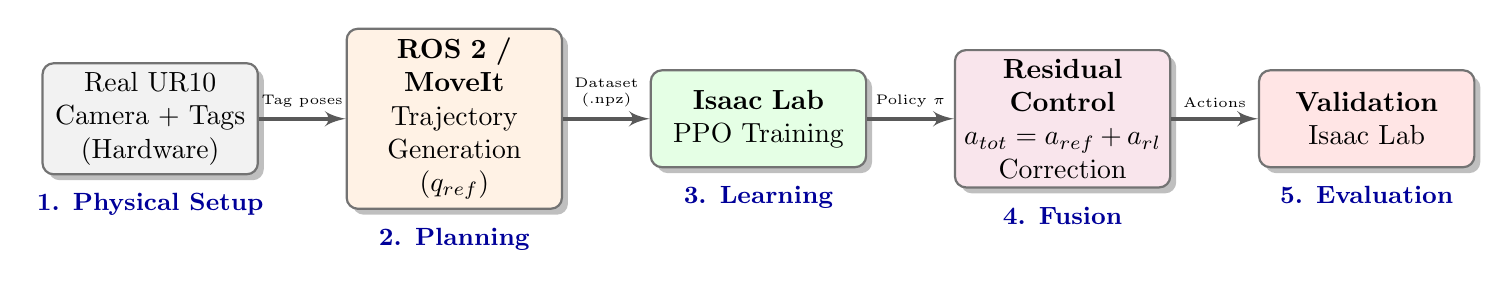
\begin{tikzpicture}[
        node distance=0.7cm and 1.1cm,
        auto,
        >=latex',
        thick,
        % Style des boîtes principales
        block/.style={
            rectangle, 
            draw=black!55, 
            fill=blue!5, 
            text width=2.5cm, 
            align=center, 
            rounded corners, 
            minimum height=3.5em,
            drop shadow
        },
        % Style des boîtes de titre (étapes)
        steptext/.style={
            font=\bfseries\small, 
            color=blue!60!black, 
            below=0.1cm
        },
        % Style des flèches
        line/.style={
            ->, 
            ultra thick, 
            color=gray!70!black
        }
    ]

    % --- ÉTAPE 1 : MATÉRIEL ---
    \node [block, fill=gray!10] (setup) {Real UR10\\Camera + Tags\\(Hardware)};
    \node [steptext] at (setup.south) {1. Physical Setup};

    % --- ÉTAPE 2 : ROS 2 ---
    \node [block, right=of setup, fill=orange!10] (ros) {\textbf{ROS 2 / MoveIt}\\Trajectory\\Generation ($q_{ref}$)};
    \node [steptext] at (ros.south) {2. Planning};

    % --- ÉTAPE 3 : ISAAC LAB ---
    \node [block, right=of ros, fill=green!10] (isaac) {\textbf{Isaac Lab}\\PPO Training\\};
    \node [steptext] at (isaac.south) {3. Learning};

    % --- ÉTAPE 4 : RÉSIDUEL ---
    \node [block, right=of isaac, fill=purple!10] (residual) {\textbf{Residual Control}\\$a_{tot} = a_{ref} + a_{rl}$\\Correction};
    \node [steptext] at (residual.south) {4. Fusion};

    % --- ÉTAPE 5 : VALIDATION ---
    \node [block, right=of residual, fill=red!10] (valid) {\textbf{Validation}\\Isaac Lab\\};
    \node [steptext] at (valid.south) {5. Evaluation};

    % --- FLÈCHES DE CONNEXION ---
    \draw [line] (setup) -- node[above, font=\tiny, text=black] {Tag poses} (ros);
    \draw [line] (ros) -- node[above, font=\tiny, align=center, text=black] {Dataset\\(.npz)} (isaac);
    \draw [line] (isaac) -- node[above, font=\tiny, text=black] {Policy $\pi$} (residual);
    \draw [line] (residual) -- node[above, font=\tiny, text=black] {Actions} (valid);

    \end{tikzpicture}
    \caption{Global project pipeline from physical setup to validation.}
    \label{fig:global_pipeline}
\end{figure}

\textbf{Stage 1: Physical Setup.} The real UR10 robot equipped with camera and AprilTags provides tag pose measurements that serve as targets for motion planning (detailed in Section 2.2).

\textbf{Stage 2: ROS 2 Planning.} MoveIt2 generates nominal trajectories ($q_{ref}$) between detected tag positions using Cartesian path interpolation. These trajectories serve as reference motions that the RL policy will learn to improve through residual corrections (detailed in Chapter 3).

\textbf{Stage 3: Isaac Lab Learning.} The dataset of reference trajectories is loaded into Isaac Lab where a PPO agent learns residual corrections in 4096 parallel simulation environments. Domain randomization introduces realistic perturbations to encourage robust policy learning (detailed in Chapter 4).

\textbf{Stage 4: Residual Control Fusion.} The learned policy produces residual actions ($a_{rl}$) that are added to the nominal actions ($a_{ref}$) to obtain the final control: $a_{tot} = a_{ref} + a_{rl}$. This additive structure ensures the policy starts from a safe baseline and only learns corrective adjustments.

\textbf{Stage 5: Validation in Isaac Lab.} After training, we compare the performance of three approaches: (1) MoveIt baseline alone (no RL), (2) RL policy alone (no MoveIt), and (3) Residual control (MoveIt + RL). This comparison demonstrates the benefit of combining classical planning with learned corrections under realistic noise and calibration errors (detailed in Chapter 5).

\subsection{Hardware Setup}

\begin{figure}[h]
\centering
\begin{overpic}[width=0.35\textwidth]{images/Robot_reel.jpg}
  \put(21,52){\colorbox{white}{\textbf{\textcolor{red}{1}}}}
  \put(26,26){\colorbox{white}{\textbf{\textcolor{blue}{2}}}}
  \put(22,13){\colorbox{white}{\textbf{\textcolor{green!60!black}{3}}}}
  \put(24,93){\colorbox{white}{\textbf{\textcolor{orange}{4}}}}
\end{overpic}
\caption{Real-world setup: (1) UR10 manipulator, (2) reference tag, (3) Workspace area, (4) Camera}
\label{fig:real_setup}
\end{figure}

The physical system (Figure \ref{fig:real_setup}) corresponds to Stage 1 of the pipeline and consists of:
\begin{itemize}
  \item \textbf{UR10 manipulator (1):} 6 degrees of freedom industrial robot for trajectory following tasks.
  \item \textbf{Reference tag (2):} AprilTag marker anchoring the world coordinate system to ensure stable and repeatable measurements across all experiments.
  \item \textbf{Workspace (3):} Defined planar area with dimensions X: [0.7m, 1.0m], Y: [-0.2m, 0.2m], Z: 0.2m fixed height. This constrained workspace simplifies the learning problem while remaining representative of real trajectory following scenarios.
  \item \textbf{Camera (4):} Webcam mounted in an eye-to-hand configuration for AprilTag detection and 3D localization of target objects.
\end{itemize}

\subsubsection{Camera and AprilTag Specifications}

\textbf{Camera hardware.} We use a Logitech C930e webcam configured at 640$\times$480 resolution running at 30 frames per second. This consumer-grade camera provides sufficient image quality for AprilTag detection while maintaining real-time performance.

\textbf{Intrinsic calibration.} The camera's intrinsic parameters (focal lengths, principal point, distortion coefficients) were calibrated using a standard checkerboard calibration pattern. The resulting camera matrix is:
\begin{equation}
K = \begin{bmatrix}
507.71 & 0 & 318.97 \\
0 & 507.01 & 237.61 \\
0 & 0 & 1
\end{bmatrix}
\end{equation}
with radial and tangential distortion coefficients modeled using the plumb\_bob model ($k_1=0.149, k_2=-0.675, p_1=-0.002, p_2=-0.001, k_3=1.382$). These parameters enable accurate 3D pose estimation from 2D image measurements.

\textbf{AprilTag configuration.} We use four AprilTag markers from the 36h11 family, each measuring 10cm $\times$ 10cm. The tag IDs are 0, 1, 2, and 3, with tag 1 serving as the reference anchor frame. The 36h11 family provides robust detection with low false positive rates while maintaining computational efficiency.

\textbf{Extrinsic calibration.} The transformation between the robot base and the reference tag (2) was obtained through manual physical measurement using a measuring tape. The measured offsets are: $\Delta x = -0.193$ m, $\Delta y = -0.255$ m, $\Delta z = -0.01$ m relative to the robot base frame. These values are encoded as a static TF transformation in the ROS 2 launch file, establishing the world coordinate frame origin. While manual calibration is less precise than automatic hand-eye calibration methods, it provides sufficient accuracy for our workspace dimensions and is straightforward to implement.

\subsection{Coordinate Frame Transformations}

\begin{figure}[h]
\centering
\includegraphics[width=0.5\textwidth]{images/Ros2_env.jpeg}
\caption{ROS2 TF visualization showing workspace boundaries and coordinate frames}
\label{fig:ros_tf}
\end{figure}

The camera (4) detects AprilTag markers and estimates their 3D positions in its local frame. To enable motion planning in the robot's coordinate system, we establish a fixed world coordinate system anchored to the reference tag (2) with a vertical offset of 21.5cm to align with the robot's base frame. 

\textbf{Importance of the reference tag (2).} This anchor frame is critical: without it, the coordinate system would drift as the camera moves or vibrates, causing inconsistent target positions. By fixing the world frame to a stationary physical marker, all measurements remain stable and repeatable—essential for precise manipulation tasks.

The transformation chain (Figure \ref{fig:ros_tf}) follows the kinematic sequence:
\begin{equation}
\text{World} \rightarrow \text{Reference Tag} \rightarrow \text{Camera} \rightarrow \text{Target Tag}
\end{equation}

Mathematically expressed as:
\begin{equation}
T_{\text{base}}^{\text{tag}} = T_{\text{base}}^{\text{ref}} \cdot T_{\text{ref}}^{\text{cam}} \cdot T_{\text{cam}}^{\text{tag}}
\end{equation}
where:
\begin{itemize}
  \item $T_{\text{cam}}^{\text{tag}}$: camera frame → detected tag (vision-based detection)
  \item $T_{\text{ref}}^{\text{cam}}$: reference tag → camera (calibrated once)
  \item $T_{\text{base}}^{\text{ref}}$: robot base → reference tag (21.5cm vertical offset)
\end{itemize}

This chain allows any detected tag position to be expressed in the robot's base frame for motion planning.


\chapter{ROS 2 / MoveIt Trajectory Generation}
\section{Objectif}
Créer un "manuel scolaire" de trajectoires parfaites pour l'IA.

\section{Stratégie Planare}
Pourquoi forcer le mouvement en 2D pour éviter l'ambiguïté de profondeur des caméras.

\section{Utilisation de MoveIt}
\subsection{Interpolation cartésienne}
Pour des droites parfaites.
\subsection{Randomisation}
Randomisation des points de départ et d'arrivée dans le cube défini (Workspace).

\section{Exportation}
Format .npz pour le transfert vers Isaac Lab.


\chapter{Isaac Lab Training Environment}
\section{Isaac Lab Environment}
The choice of \textbf{Isaac Lab} is justified by its capability for \textit{massive parallelization} on GPU.
In our configuration, we instantiate \textbf{4096 simultaneous environments} ($N_{envs} = 4096$). These environments are capable of iteratively simulating various parameter configurations, including system noise and environmental randomization.
This allows collecting millions of experience samples in a few minutes, drastically accelerating training compared to real-time or 
standard CPU-based simulation.

\section{Synthetic Perception \& Noise}
To bridge the \textit{Sim2Real} gap (Reality Gap), real-world imperfections are explicitly modeled in the simulator. These perturbations affect both the agent's perception and the physical dynamics:

\begin{itemize}
    \item \textbf{Camera Model (Pinhole)}: A virtual camera is placed with realistic intrinsic parameters ($f_x=491.6, f_y=488.0$) and a defined extrinsic pose.
    \item \textbf{Projection Noise (Visual Jitter)}: A re-projection error is added to the camera measurements as Gaussian noise on the pixels ($\sigma_{pixel} = 0.355$).
    \item \textbf{3D Measurement Noise (XYZ Jitter)}: Direct Gaussian noise is added to the cartesian position measurement of the end-effector to simulate depth estimation noise ($\sigma_{xyz} = 2$ mm).
    \item \textbf{Calibration Error (Extrinsic Bias)}: A random bias is added to the camera pose, sampled uniformly within a sphere of radius $\pm 2$ cm ($b_{ext} \sim \mathcal{U}(-0.02, 0.02)$ m). This bias is resampled at each episode.
    \item \textbf{Target Noise (Goal Uncertainty)}: The desired target position $EE_{des}$ observed by the agent is corrupted by Gaussian noise ($\sigma_{target} = 2$ mm), simulating uncertainty in the tracking objective.
    \item \textbf{Latency (Action Delay)}: Communication delay is simulated by delaying action application by \textbf{1 to 3 simulation steps} (approx. 17--50 ms).
    \item \textbf{Dynamics Randomization}: To account for physical discrepancies, the following parameters are randomized per episode:
    \begin{itemize}
        \item \textbf{Payload Mass}: A random mass is attached to the end-effector ($m_{load} \sim \mathcal{U}(0.0, 0.5)$ kg).
        \item \textbf{Joint Damping}: Scaled by a multiplicative factor $\in [0.8, 1.2]$.
        \item \textbf{Friction}: Surface friction coefficients are randomized (Static $\mu_s \in [0.6, 1.2]$, Dynamic $\mu_d \in [0.5, 1.0]$).
    \end{itemize}
\end{itemize}
\section{AI Modeling}

\subsection{Inputs (Observations)}
The observation space, with a dimension of 40, consists of:
\begin{enumerate}
    \item \textbf{Proprioception}: Joint positions $q \in \mathbb{R}^6$, Joint velocities $\dot{q} \in \mathbb{R}^6$.
    \item \textbf{Reference}: Reference joint positions $q_{ref} \in \mathbb{R}^6$ and tracking error $e_q = q - q_{ref} \in \mathbb{R}^6$.
    \item \textbf{Task (Cartesian Space)}:
    \begin{itemize}
        \item Measured end-effector position (noisy) $EE_{meas} \in \mathbb{R}^3$.
        \item Desired target position $EE_{des} \in \mathbb{R}^3$.
        \item Cartesian error $e_{EE} = EE_{meas} - EE_{des} \in \mathbb{R}^3$ and its norm $\|e_{EE}\| \in \mathbb{R}^1$.
    \end{itemize}
    \item \textbf{Previous State}: Last applied actions $a_{t-1} \in \mathbb{R}^6$.
\end{enumerate}

\subsection{Outputs (Actions)}
The neural network predicts \textbf{additive joint corrections} (residuals).
These values are normalized between $[-1, 1]$ by the $\tanh$ activation function, then scaled by a factor $k_{scale} = 0.05$.
This limits the agent's authority to $\pm 0.05$ rad ($\approx 2.8^\circ$) per time step around the reference trajectory, ensuring movement safety and stability.

\section{Reward Function}
The reward function is designed to maximize precision while minimizing energy and vibrations. It uses an exponential kernel to be dense and bounded within $[0, 1]$.

Simplified mathematical formulation ($r_t$):
\begin{equation}
    r_t = \underbrace{\exp\left(-\frac{\|e_{pos}\|^2}{\sigma_{pos}^2}\right)}_{\text{Precision}}
    - \underbrace{\lambda_{v} \|\dot{x}_{ee}\|^2}_{\text{Smoothness}}
    - \underbrace{\lambda_{a} \|\ddot{x}_{ee}\|^2}_{\text{Stability}}
    + r_{bonus}
\end{equation}

\begin{itemize}
    \item \textbf{Precision Term}: Rewards proximity to the cartesian target ($\sigma_{pos} = 0.02$ m).
    \item \textbf{Regularization Penalties}:
    \begin{itemize}
        \item End-effector velocity ($\lambda_{v}=0.03$) to avoid jerky movements.
        \item End-effector acceleration ($\lambda_{a}=0.01$) to reduce vibrations (jitter).
    \end{itemize}
    \item \textbf{Bonus}: A constant bonus ($0.5$) is awarded if the error is below a critical threshold (2 cm), incentivizing the agent to maintain final precision.
\end{itemize}

\chapter{Validation \& Results}
\section{Validation in Isaac Lab }
To assess the performance of our residual reinforcement learning approach, we first evaluated the learned policy directly in the Isaac Lab 
training environment. This controlled simulation setting allows us to precisely measure the improvement brought by the AI agent compared to
 a Open-Loop controller under localized perturbations.

\subsection{Experimental Control Modes: Open-Loop vs. AI Closed-Loop}
Before presenting the quantitative results, we distinguish the two control strategies evaluated in this validation phase:

\begin{itemize}
    \item \textbf{Open-Loop (Baseline):} The robot executes the trajectory theoretically planned by MoveIt. In a perfect simulation, this would be accurate. However, in our "Sim-to-Real" validation scenarios, we introduce calibration errors (offset between the camera and the robot base) and sensor noise. In open-loop, the robot blindly follows the plan without correcting for these discrepancies, leading to significant end-effector errors.
    
    \item \textbf{Closed-Loop RL (AI):} This is the proposed residual learning approach. The AI agent acts as a high-frequency feedback controller (60Hz). It continuously monitors the \textit{observed} state (proprioception + noisy vision) and the tracking error. Unlike the baseline, the AI "closes the loop" by injecting real-time joint corrections ($\Delta q$) to minimize the distance to the perceived target. This allows it to dynamically compensate for the static calibration errors and filter out high-frequency sensor noise.
\end{itemize}

The achieved success rate exceeds 95\% on a test set comprising random trajectories with perception noise and simulated calibration error. This validates that the agent has successfully learned to correct the trajectories from the MoveIt planner.

\begin{figure}[htbp]
    \centering
    \includegraphics[width=0.9\textwidth]{images/table_summary.png}
    \caption{Performance summary comparing open-loop and closed-loop RL approaches. The RL policy achieves 69.7\% improvement in mean error, 55.6\% in max error, and 71.4\% in standard deviation.}
    \label{fig:performance_summary}
\end{figure}

Figure~\ref{fig:performance_summary} presents quantitative metrics comparing open-loop and closed-loop RL approaches:
\begin{itemize}
    \item \textbf{Mean error}: 28.37mm $\rightarrow$ 8.58mm (69.7\% improvement)
    \item \textbf{Max error}: 52.03mm $\rightarrow$ 23.08mm (55.6\% improvement)
    \item \textbf{Standard deviation}: 15.36mm $\rightarrow$ 4.39mm (71.4\% improvement)
    \item \textbf{Speed}: Average 187.9 mm/s, peak 587.5 mm/s
\end{itemize}
All error metrics show $>$50\% improvement, confirming the effectiveness of the RL correction approach.

\begin{figure}[htbp]
    \centering
    \includegraphics[width=0.95\textwidth]{images/fig1_error_comparison.png}
    \caption{Tracking accuracy comparison: Open-Loop vs Closed-Loop RL. The red curve shows the open-loop position error (mean=28.4mm, max=52.0mm), while the green curve demonstrates the closed-loop RL correction (mean=8.6mm, max=23.1mm), representing a 70\% improvement.}
    \label{fig:error_comparison}
\end{figure}

Figure~\ref{fig:error_comparison} shows the position error norm over time. The red curve (open-loop) exhibits mean error of 28.4mm with peaks exceeding 52mm, particularly during rapid direction changes at t=1.0s and t=3.8s. The green curve (closed-loop RL) maintains mean error of 8.6mm with maximum error below 23mm, representing a 70\% improvement. The RL agent anticipates errors and attenuates disturbances without introducing oscillations.

\begin{figure}[htbp]
    \centering
    \includegraphics[width=0.95\textwidth]{images/fig2_ee_position_x.png}
    \caption{Trajectory tracking on X-axis. The blue dashed line represents the desired trajectory, the orange dotted line shows the observed trajectory with noise, and the green solid line indicates the actual trajectory executed by the RL agent.}
    \label{fig:trajectory_x}
\end{figure}

Figure~\ref{fig:trajectory_x} shows end-effector position along the X-axis. The blue dashed line represents the ideal reference trajectory, the orange dotted line shows noisy observations with sensor noise and calibration errors, and the green solid line indicates the actual executed trajectory. The RL agent tracks the reference with 5.3mm average error on X-axis, demonstrating robustness to observation noise by filtering rather than blindly following noisy measurements.

\begin{figure}[htbp]
    \centering
    \includegraphics[width=0.95\textwidth]{images/fig4_joint_j4_strategy.png}
    \caption{Joint J4 (wrist\_1) position comparison. Top: open-loop tracking shows deviation from reference. Bottom: closed-loop RL applies a bias of +0.63° on J4 to improve end-effector accuracy.}
    \label{fig:joint_j4}
\end{figure}

Figure~\ref{fig:joint_j4} reveals the RL correction strategy at joint level for J4 (wrist\_1). Top panel: open-loop tracking follows the reference perfectly but leads to end-effector errors. Bottom panel: the RL policy systematically applies a +0.63\textdegree\ bias to J4. The gap between the reference (blue dashed) and RL-corrected target (orange dotted) shows this proactive compensation. This consistent bias compensates for systematic errors (gravity, friction, calibration) and exploits kinematic redundancy to improve end-effector accuracy without compromising motion quality.

\begin{figure}[htbp]
    \centering
    \includegraphics[width=0.9\textwidth]{images/fig3_ee_speed.png}
    \caption{End-effector speed during trajectory execution. Average speed: 187.9 mm/s, maximum speed: 587.5 mm/s.}
    \label{fig:ee_speed}
\end{figure}

Figure~\ref{fig:ee_speed} shows the end-effector velocity profile with average speed of 187.9 mm/s and peak of 587.5 mm/s at t=2.0s. The smooth profile without high-frequency oscillations indicates stable control. The velocity modulation demonstrates an emergent speed-accuracy trade-off learned during training, where the agent adaptively adjusts speed based on trajectory requirements while maintaining safety limits.

\section{Limitations of this validation}
Although the results in Isaac Lab are promising, this validation remains a "Sim-to-Sim" evaluation within the same physics engine (PhysX). 
The main risk is that the policy may have learned to exploit simulation-specific artifacts (numerical errors, simplified friction model) that do not exist in reality.
To ensure true robustness before real-world deployment, it is crucial to test the policy in a physically different environment.







% \chapter{Sim-to-Real Transfer}
% \input{chapters/sim_to_real}

\chapter{Conclusion \& Perspectives}
\section{Summary of Contributions}

This work successfully demonstrated a hybrid approach combining classical motion planning with reinforcement learning for robust trajectory tracking on a UR10 manipulator. The key contributions include:

\textbf{System Integration.} We established a complete pipeline connecting ROS 2/MoveIt for trajectory generation, Isaac Lab for massively parallel PPO training (4096 environments), and a residual learning architecture where learned corrections enhance rather than replace classical planning. This integration proves that traditional robotics tools can be effectively combined with modern deep RL frameworks.

\textbf{Residual Learning Architecture.} The residual control formulation $a_{total} = a_{ref} + a_{residual}$ preserves safety guarantees from MoveIt's collision-free planning while enabling learned adaptations to perception errors and calibration inaccuracies. This approach significantly reduces the learning complexity compared to end-to-end RL by constraining the policy to learn only small corrective actions ($\pm 0.05$ rad/s).

\textbf{Domain Randomization Strategy.} We implemented comprehensive noise modeling including sensor jitter ($\pm 2$mm), calibration errors ($\pm 2$cm), action delays (17--50ms), and dynamics randomization (payload, friction, damping). This multi-layer perturbation strategy forces the policy to generalize beyond perfect simulation conditions.

\textbf{Validation Results.} The trained policy achieved strong performance in Isaac Lab validation: 69.7\% improvement in mean tracking error (28.4mm $\rightarrow$ 8.6mm), 55.6\% reduction in maximum error (52.0mm $\rightarrow$ 23.1mm), and 71.4\% improvement in consistency (standard deviation: 15.4mm $\rightarrow$ 4.4mm). The agent learned emergent strategies such as systematic joint bias compensation (+0.63° on J4) and adaptive speed modulation.

\section{Limitations and Lessons Learned}

\textbf{Sim-to-Sim Validation Only.} The current validation remains within Isaac Lab's PhysX engine. While domain randomization improves robustness, there is a risk that the policy exploited simulation-specific artifacts (numerical precision, simplified contact models, deterministic dynamics) that differ from physical reality. This represents the primary limitation of this work.

\textbf{Time Constraints.} The original objective was full sim-to-real transfer on the physical UR10. However, time limitations prevented extensive real-world testing. Deploying learned policies on physical systems requires careful safety protocols, failure recovery mechanisms, and iterative tuning—processes that demand significant experimentation time beyond the scope of this project.

\textbf{Calibration Dependency.} Although the policy is trained to handle calibration errors up to $\pm 2$cm, deployment success depends critically on initial calibration quality. If real-world errors exceed the training distribution, performance degradation is expected. This highlights the importance of good initial calibration even when using adaptive controllers.

\section{Future Work and Perspectives}

If given additional time, several validation steps would strengthen confidence in real-world transferability:

\textbf{Sim-to-Sim Transfer: Isaac Lab $\rightarrow$ MuJoCo.} The immediate next step is evaluating the trained policy in a physically different simulator (MuJoCo) with distinct physics engines, contact solvers, and numerical integrators. Success in cross-simulator transfer would provide strong evidence that the policy learned generalizable control strategies rather than simulation-specific heuristics. MuJoCo's different friction model and more accurate contact dynamics would serve as an intermediate reality gap test before attempting real robot deployment.

\textbf{Physical Robot Deployment.} The ultimate objective is deployment on the physical UR10. This transition from simulation to reality represents the final validation step, where the policy would face true sensor noise, unmodeled dynamics, and real-world uncertainties that cannot be perfectly captured in simulation. Successful deployment would require careful safety protocols and progressive testing to ensure reliable operation.

\textbf{Extended Scenarios.} Beyond trajectory following, the learned residual control could be extended to more complex manipulation tasks involving object grasping, dynamic obstacle avoidance, and contact-rich interactions. The current framework provides a solid foundation that could be enriched with additional perception modalities (RGB-D cameras, force-torque sensors) and more sophisticated task specifications.

\section{Conclusion}

This work demonstrates that residual reinforcement learning offers a promising middle ground between classical motion planning and end-to-end learned control. By combining the safety and interpretability of traditional planners with the adaptability of deep RL, we achieve robust trajectory tracking under realistic perception noise and calibration errors—at least within simulation.

The strong validation results in Isaac Lab (>69\% error reduction) confirm the technical viability of the approach. However, the true test lies in physical deployment, which remains the natural continuation of this work. With proper safety protocols, cross-simulator validation, and iterative refinement, sim-to-real transfer is an achievable next step that would validate the practical utility of this hybrid architecture for real-world robotic manipulation.


% Uncomment the lines below when you add citations to your document
% \bibliographystyle{plain}
% \bibliography{references}

\end{document}
